\documentclass[a4paper,12pt]{article}
\usepackage{pgf,tikz,pgfplots}
\usepackage{tikz}
\usetikzlibrary{cd}
\pgfplotsset{compat=1.15}
\usetikzlibrary{arrows}
\usepackage{amsmath,amssymb}

\newcommand{\CB}{\mathcal{B}}

\begin{document}

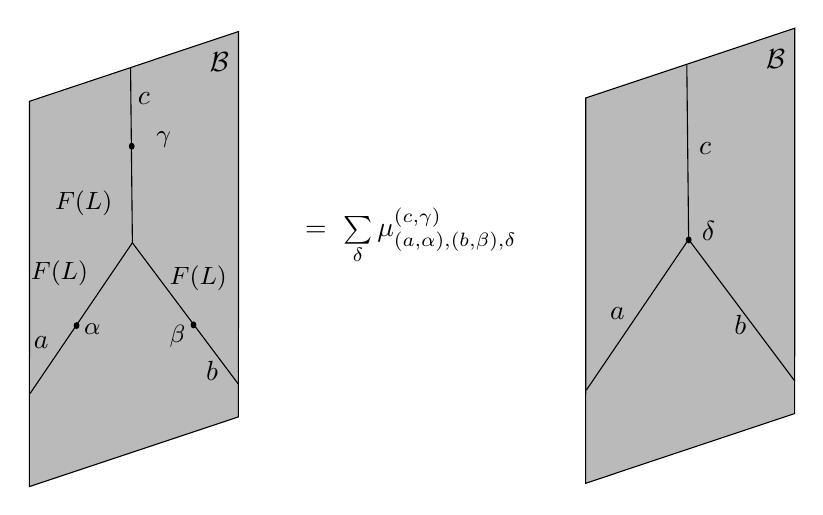
\begin{tikzpicture}[x=0.75pt,y=0.75pt,yscale=-0.8,xscale=0.8]

\draw  [color={rgb, 255:red, 0; green, 0; blue, 0 }  ,draw opacity=1 ][fill={rgb, 255:red, 74; green, 74; blue, 74 }  ,fill opacity=0.38 ] (116.59,387.85) -- (116.63,155.8) -- (242.51,113.8) -- (242.46,345.85) -- cycle ;
\draw    (117,331.75) -- (178.6,241.01) ;
\draw    (242.5,326.25) -- (178.6,241.01) ;
\draw    (178.6,241.01) -- (177.5,135.75) ;
\draw  [color={rgb, 255:red, 0; green, 0; blue, 0 }  ,draw opacity=1 ][fill={rgb, 255:red, 0; green, 0; blue, 0 }  ,fill opacity=1 ] (213.99,290.47) .. controls (213.99,289.51) and (214.62,288.74) .. (215.4,288.74) .. controls (216.18,288.74) and (216.81,289.51) .. (216.81,290.47) .. controls (216.81,291.42) and (216.18,292.2) .. (215.4,292.2) .. controls (214.62,292.2) and (213.99,291.42) .. (213.99,290.47) -- cycle ;
\draw  [color={rgb, 255:red, 0; green, 0; blue, 0 }  ,draw opacity=1 ][fill={rgb, 255:red, 0; green, 0; blue, 0 }  ,fill opacity=1 ] (143.59,290.87) .. controls (143.59,289.91) and (144.22,289.14) .. (145,289.14) .. controls (145.78,289.14) and (146.41,289.91) .. (146.41,290.87) .. controls (146.41,291.82) and (145.78,292.6) .. (145,292.6) .. controls (144.22,292.6) and (143.59,291.82) .. (143.59,290.87) -- cycle ;
\draw  [color={rgb, 255:red, 0; green, 0; blue, 0 }  ,draw opacity=1 ][fill={rgb, 255:red, 0; green, 0; blue, 0 }  ,fill opacity=1 ] (176.79,182.87) .. controls (176.79,181.91) and (177.42,181.14) .. (178.2,181.14) .. controls (178.98,181.14) and (179.61,181.91) .. (179.61,182.87) .. controls (179.61,183.82) and (178.98,184.6) .. (178.2,184.6) .. controls (177.42,184.6) and (176.79,183.82) .. (176.79,182.87) -- cycle ;
\draw  [color={rgb, 255:red, 0; green, 0; blue, 0 }  ,draw opacity=1 ][fill={rgb, 255:red, 74; green, 74; blue, 74 }  ,fill opacity=0.38 ] (451.59,385.85) -- (451.63,153.8) -- (577.51,111.8) -- (577.46,343.85) -- cycle ;
\draw    (452,329.75) -- (513.6,239.01) ;
\draw    (577.5,324.25) -- (513.6,239.01) ;
\draw    (513.6,239.01) -- (512.5,133.75) ;
\draw  [color={rgb, 255:red, 0; green, 0; blue, 0 }  ,draw opacity=1 ][fill={rgb, 255:red, 0; green, 0; blue, 0 }  ,fill opacity=1 ] (512.19,239.28) .. controls (512.19,238.32) and (512.82,237.55) .. (513.6,237.55) .. controls (514.38,237.55) and (515.01,238.32) .. (515.01,239.28) .. controls (515.01,240.24) and (514.38,241.01) .. (513.6,241.01) .. controls (512.82,241.01) and (512.19,240.24) .. (512.19,239.28) -- cycle ;

% Text Node
\draw (223.7,125.1) node [anchor=north west][inner sep=0.75pt]  [font=\normalsize]  {$\CB$};
% Text Node
\draw (117.73,295.72) node [anchor=north west][inner sep=0.75pt]    {$a$};
% Text Node
\draw (221.49,310.99) node [anchor=north west][inner sep=0.75pt]    {$b$};
% Text Node
\draw (180.31,149.18) node [anchor=north west][inner sep=0.75pt]    {$c$};
% Text Node
\draw (130.41,208.13) node [anchor=north west][inner sep=0.75pt]  [font=\small]  {$F( L)$};
% Text Node
\draw (115.87,250.14) node [anchor=north west][inner sep=0.75pt]  [font=\small]  {$F( L)$};
% Text Node
\draw (199.49,253.03) node [anchor=north west][inner sep=0.75pt]  [font=\small]  {$F( L)$};
% Text Node
\draw (281,218.4) node [anchor=north west][inner sep=0.75pt]    {$=\ \sum\limits_{\delta } \mu _{( a,\alpha ) ,( b,\beta ),\delta}^{( c,\gamma )  }$};
% Text Node
\draw (148,288.4) node [anchor=north west][inner sep=0.75pt]  [font=\small]  {$\alpha $};
% Text Node
\draw (199.48,289.05) node [anchor=north west][inner sep=0.75pt]  [font=\small]  {$\beta $};
% Text Node
\draw (191.5,172.4) node [anchor=north west][inner sep=0.75pt]  [font=\small]  {$\gamma $};
% Text Node
\draw (558.7,123.1) node [anchor=north west][inner sep=0.75pt]  [font=\normalsize]  {$\CB$};
% Text Node
\draw (464.73,278.72) node [anchor=north west][inner sep=0.75pt]    {$a$};
% Text Node
\draw (539.49,282.99) node [anchor=north west][inner sep=0.75pt]    {$b$};
% Text Node
\draw (518.31,179.18) node [anchor=north west][inner sep=0.75pt]    {$c$};
% Text Node
\draw (520,226.4) node [anchor=north west][inner sep=0.75pt]    {$\delta $};


\end{tikzpicture}

\end{document}